\section{January 2021}
{\sffamily{Lorem Ipsum Dolor Sit Amet.Lorem Ipsum Dolor Sit Amet.Lorem Ipsum Dolor Sit Amet.Lorem Ipsum Dolor Sit Amet.Lorem Ipsum Dolor Sit Amet.Lorem Ipsum Dolor Sit Amet.Lorem Ipsum Dolor Sit Amet.Lorem Ipsum Dolor Sit Amet.Lorem Ipsum Dolor Sit Amet.Lorem Ipsum Dolor Sit Amet. Lorem Ipsum Dolor Sit Amet.Lorem Ipsum Dolor Sit Amet.}}
\thispagestyle{empty}
\newpage
%------------------------------------------------------------
\begin{mathbox}{\text{\subsection{A Simple Proof}}}
{Are there infinitely many prime numbers? If yes, how do we prove they exist?\\
Here's a simple proof.\\
{Assume} we have only $n$ prime numbers; $P_1, P_2, P_3, \dots P_n$.
\begin{align*}
\text{Let}~N = P_1 \cdot P_2 \cdot P_3 \dots P_n + 1
\end{align*}
$N$ {isn't divisible} by any of the primes $P_1, P_2, P_3, \dots P_n$\footnote{Prime numbers start from $2$ and $N$ is the LCM of all the prime numbers added to $1$.}  which implies $N$'s {prime factorisation} is $N \times 1$. $N$ being prime {contradicts} our initial assumption.\\
Thus, there exist infinite primes.}
\end{mathbox}
%------------------------------------------------------------
\begin{phybox}{\text{\subsection{Are we down to the Least Hierarchical Particle?}}}
{Atoms are divisible, but are electrons, protons and neutrons?. A {quark} is an elementary particle and a fundamental constituent of matter. Quarks combine to form particles called hadrons. All commonly observable matter is composed of {up quarks, down quarks and electrons}. Due to a phenomenon called "Colour Confinement", quarks are never found existing individually, they can be found only composing {hadrons}, which include {baryons} (protons and neutrons) and {mesons}, or in {quark–gluon plasma}. They are the only elementary particles in the Standard Model of particle physics to experience all four fundamental interactions (electromagnetic force, gravitation, strong forces, and weak forces).\\
Quarks are of 6 types/flavours:
\begin{itemize}
\vspace{-0.5em}
    \item{Up}
\vspace{-0.5em}
    \item{Down}
\vspace{-0.5em}
    \item{Charm}
\vspace{-0.5em}
    \item{Strange}
\vspace{-0.5em}
    \item{Top}
\vspace{-0.5em}
    \item{Bottom}
\vspace{-0.5em}
\end{itemize}
Up and down quarks have the lowest masses and such heavier quarks rapidly change into up and down quarks through the process of particle decay. Up and down quarks are generally stable and the most common in the universe, whereas strange, charm, bottom, and top quarks can only be produced in high energy collisions (such as those in particle accelerators like those found at CERN).}
\end{phybox}
%------------------------------------------------------------
\begin{chembox}{\text{\subsection{Quantum Numbers (Not a new System!?)}}}
{In chemistry and quantum physics, quantum numbers describe values of conserved quantities in the dynamics of a quantum system. 
An important aspect of quantum mechanics is the quantization of many observable quantities of interest. In particular, this leads to quantum numbers that take values in discrete sets of integers or half-integers\footnote{Numbers of the form $\frac{2n+1}{2}$}; although they approach infinity in some cases. Quantum numbers often describe specifically the energy levels of electrons in atoms, but other possibilities include angular momentum, spin, etc. An important family is flavour quantum numbers – internal quantum numbers which determine the type of a particle and its interactions with other particles through the fundamental forces. A system can have one or more quantum numbers; it is thus difficult to list all possible quantum numbers.\\
Four quantum numbers can describe an electron in an atom completely:
\begin{itemize}
    \item{Principal quantum number $(n)$}
    \item{Azimuthal quantum number $(l)$}
    \item{Magnetic quantum number $(m)$}
    \item{Spin quantum number $(s)$}
\end{itemize}
Also, the question of how many quantum numbers are needed to describe any given system has no universal answer; for each system, one must find the answer by performing a full analysis of the system. The most prominent system of nomenclature spawned from the molecular orbital theory of Friedrich Hund and Robert S. Mulliken, which incorporates Bohr energy levels as well as observations about electron spin. This model describes electrons using the above mentioned quantum numbers. It is also the common nomenclature in the classical description of nuclear particle states (e.g. protons and neutrons).}
\end{chembox}
%------------------------------------------------------------
\begin{mathbox}{\text{\subsection{Exponentiation^{-1}}}}
{The {logarithm} function (denoted by $\log$) is the {inverse} function of {exponentiation}. It denotes the {exponent/power} to which the {'base'} has been raised to in a number. Here's an example;
\begin{align*}
    \text{Let } x = a^b. \text{ This implies} \log_a (x) = b
\end{align*}
The logarithm of $x$ to the base $a$ can be a {whole number, decimal number, irrational number} or even a {complex number} depending on its value. Often, log graph are used to make growth, forecast and even the number of cases during a pandemic. Logarithms involving complex numbers\footnote{\sffamily${\sqrt{-x}, \sqrt[3]{-x}, \dots}$} $(i)$ can be plotted on the real-complex plane.
\begin{flushleft}
\begin{tikzpicture}
\begin{axis}[
    axis lines = left,
    xlabel = $x$,
    ylabel = {$\ln(x)$},
]
\addplot [
    domain=0:100, 
    samples=1000, 
    color=Red,
]
{ln(x)};
\addlegendentry{$\log_e(x) = \ln{x}$}
\end{axis}
\end{tikzpicture}
\end{flushleft}
\begin{flushleft}
\begin{tikzpicture}
\begin{axis}[
    axis lines = left,
    xlabel = $x$,
    ylabel = {$\log_2(x)$},
]
\addplot [
    domain=0:100, 
    samples=1000, 
    color=Red,
]
{log2(x)};
\addlegendentry{$\log_2(x)$}
\fill (2,1)  circle[radius=1pt, color=blue];
\fill (4,2)  circle[radius=1pt, color=blue];
\fill (8,3)  circle[radius=1pt, color=blue];
\fill (16,4)  circle[radius=1pt, color=blue];
\fill (32,5)  circle[radius=1pt, color=blue];
\fill (64,6)  circle[radius=1pt, color=blue];
\end{axis}
\end{tikzpicture}
\end{flushleft}
These are examples log-graphs to the base $e$\footnote{Euler's constant; $e = 2.71$} and $2$\footnote{The points in the $\log_2(x)$ graph represent the points where the value of $\log_2(x)$ is an integer, i.e when $x$ is a power of 2}.}
\end{mathbox}
%------------------------------------------------------------
\begin{phybox}{\text{\subsection{Vectors!}}}
{Per definition, a vector is an element of a vector space (a set containing vectors). Essentially, a vector is any quantity represented taking into consideration both its direction and its magnitude. Vectors are represented by drawing a ray over them (preferably in their direction); i.e. $a$ vectors as  $\Vec{a}$. 
A vector's output is decided by these 2 constituents;
\begin{itemize}
    \item{Magnitude; represented $||\Vec{a}||$ or $|\Vec{AB}|$ is the technically the length of the vector. Suppose 
    \begin{align*}
        \Vec{a} = m_1 \hat{a_1} + m_2 \hat{a_2} + m_3 \hat{a_3} + \dots m_n \hat{a_n}
    \end{align*} 
     where $\hat{a_1}, \hat{a_2}, \hat{a_3}, \dots \hat{a_n}$ represent the unit vectors in the $n$ different axes/dimensions and $m_1, m_2, m_3, \dots m_n$ are the respective coefficients,
    its magnitude is
    \begin{align*}
    \sqrt{m_1^2 + m_2^2 + m_3^2 + \dots m_n^2}
    \end{align*}}
    \item{Direction; either positive or negative.}
\end{itemize}
This is an example of a vector ($\Vec{a}$) with co-ordinates $x', y'$ and $z'$ where $\Vec{x}, \Vec{y}$ and $\Vec{z}$ are the unit vectors;
\begin{center}
\begin{tikzpicture}[scale=3,tdplot_main_coords]
	\draw[thick,->] (0,0,0) -- (1,0,0) node[anchor=north east]{$x$};
	\draw[thick,->] (0,0,0) -- (0,1,0) node[anchor=north west]{$y$};
	\draw[thick,->] (0,0,0) -- (0,0,1) node[anchor=south]{$z$};
	\tdplotsetcoord{O}{0}{0}{0}
	\tdplotsetcoord{P}{1}{1}{1}
	\draw[tdplot_rotated_coords,color=red,thick,->] (0,0,0)
	-- (.5,.5,.5) node[anchor=south]{$\Vec{a}$};
	\tdplotsetthetaplanecoords{70}
	\draw[tdplot_rotated_coords,color=blue,thick,->] (0,0,0)
	-- (.5,0,0) node[anchor=north]{$x'$};
	\draw[tdplot_rotated_coords,color=blue,thick,->] (0,0,0)
	-- (0,.5,0) node[anchor=east]{$y'$};
	\draw[tdplot_rotated_coords,color=blue,thick,->] (0,0,0)
	-- (0,0,.5) node[anchor=west]{$z'$};
\end{tikzpicture}
\end{center}
Vectors can be added to, subtracted from, multiplied or divided by another vector. Hence, $\Vec{a}$ is actually the sum of three vectors $x', y'$ and $z'$\footnote{We call the vectors formed by the points $x', y', z'$ the way they are named. But this isn't the case always. You will later come to know why its true in this case.\\
If you want to know right now, Hint: The vector's start is the origin $(0,0,0)$ } i.e
\begin{align*}
    \Vec{a} = \Vec{x'} + \Vec{y'} + \Vec{z'}
\end{align*}
There are a couple of laws and formulas that govern the arithmetic operations on vectors. Keep reading for those.}
\end{phybox}
%------------------------------------------------------------
\begin{phybox}{\text{\subsection{Arithmetic Operations on Vectors}}}
{The triangle rule of vector addition describes how we can add vectors;
\begin{center}
\begin{tikzpicture}[scale=3,tdplot_main_coords]
	\draw[thick,->, color=blue] (0,0,0) -- (.5,0,0) node[anchor=south east]{$\Vec{a}$};
	\draw[thick,->, color=blue] (0,0,0) -- (0,.5,.5) node[anchor=east]{$\Vec{b}$};
	\draw[thick,->, color=red] (0,0,0) -- (.5,.5,.5) node[anchor=south]{$\Vec{a} + \Vec{b}$};
	\draw[dashed, opacity=0.3] (.5,0,0) -- (0,.5,.5) node[anchor=west];
\end{tikzpicture}
\end{center}
the vector from the tip of is resultant of the sum of $\Vec{a}$ and $\Vec{b}$.
\begin{itemize}
    \item{The magnitude of $\Vec{a} + \Vec{b}$ is 
    \begin{align*}
        \sqrt{a^2 + 2ab \cos\theta + b^2}
    \end{align*} where $a$ and $b$ are the magnitudes of $\Vec{a}$ and $\Vec{b}$ respectively, and $\theta$ is the angle between $\Vec{a}$ and $\Vec{b}$}
    \item{If the angle made by $\Vec{a} + \Vec{b}$ with $\Vec{a}$ is $\alpha$, then \begin{align*}
        \tan\alpha = \frac{b \sin \theta}{a + b \cos\theta}
    \end{align*}}
\end{itemize}
Coming to subtraction, it's the same but you take the negative value of the vector you subtract and add;
\begin{center}
\begin{tikzpicture}[scale=3,tdplot_main_coords]
	\draw[thick,->, color=blue] (0,0,0) -- (.5,0,0) node[anchor=south east]{$\Vec{a}$};
	\draw[thick,dashed, color=blue] (0,0,0) -- (0,.5,.5) node[anchor=east]{$\Vec{b}$};
	\draw[thick,->, color=blue] (0,0,0) -- (0,-.5,-.5) node[anchor=east]{$\Vec{-b}$};
	\draw[thick,->, color=red] (0,0,0) -- (.5,-.5,-.5) node[anchor=west]{$\Vec{a} - \Vec{b}$};
	\draw[dashed, opacity=0.3] (.5,0,0) -- (0,-.5,-.5) node[anchor=west];
\end{tikzpicture}
\end{center}
We can also multiply a vector by a scalar. If we have $\Vec{a}$ with magnitude $a$ and direction, multiplying it by a scalar $m$ with magnitude $0.5$ will give a new vector with magnitude $\frac{a}{2}$. Similarly, if we take 3 which is a scalar and multiply it by a $\Vec{b}$, you get a new vector 3 times as long as $\Vec{b}$. As a more physical example, the gravitational force on an object is a vector with its magnitude depending on a scalar; mass. If the mass of the object is doubled, the gravitational force is doubled as well.
\begin{center}
    If $\Vec{a} = x \hat{i} + y \hat{j} + z \hat{k}$\\
    then $|\Vec{b}| = 2 \times |a| = 2 \cdot \sqrt{x^2 + y^2 + z^2}$
\end{center}
\begin{center}
\begin{tikzpicture}[scale=3,tdplot_main_coords]
    \draw[thick,->] (0,0,0) -- (.8,0,0) node[anchor=north east]{$x$};
	\draw[thick,->] (0,0,0) -- (0,.8,0) node[anchor=north east]{$y$};
	\draw[thick,->, color=blue] (0,0,0) -- (.3,.3,.3) node[anchor=south east]{$\Vec{a}$};
	\draw[thick,->, color=red] (0,0,0) -- (.6,.6,.6) node[anchor=south east]{$2 \Vec{a}$};
\end{tikzpicture}
\end{center}
The same goes with division.}
\end{phybox}
%------------------------------------------------------------
\begin{mathbox}{\text{\subsection{Sets; Colloquially, Groups!}}}
{In mathematics, a set is a well-defined collection of distinct elements\footnote{Elements are the distinct or same values that can be numbers, letters, words, codes, etc.} or members. Sets' elements can be anything; literally! They can define points or co ordinates, names, letters, geometrical shapes, equations, lines, constants, variables or even other sets. We have a few basic operations involving sets that resemble the four arithmetic operations.\\
\textbf{Set Notation:}\\
A set is defined by enclosing its elements within two parentheses (open and close) in the form "\{Element 1, Element 2, Element 3, \dots\}" where the elements are separated by commas.\\
We can also include other sets inside a subset in these two ways "$\{\{S^1_{e_1}, S^1_{e_2}, \dots\}, \{S^2_{e_1}, S^2_{e_2}, \dots\}, \dots\}$" or "$\{S^1, S^2, \dots\}$" where $S^1, S^2, \dots$ represent the different sets and $e_!, e_2,\dots$ represent the different elements in each of the sets.\\
\textbf{Subsets and Supersets:}\\
A subset is a collection of elements as well, but all of its elements are part of a bigger or equal set\footnote{Here, bigger and equal refer to the number of elements in the sets.}. For example we define $S = \{1, 2, 3, 4, 5, 6\}$, and $SS = \{1, 2, 3, 5\}$. We say $SS$ is a subset of $S$ since all of its elements are a part of $S$. This is conveyed mathematically in the form; 
\begin{align*}
    SS \subset S
\end{align*} where $\subset$ is the symbol for "subset".\\
A superset is the exact inverse and we can say $S$ is a superset of $SS$. It's represented as; 
\begin{align*}
S \supset SS    
\end{align*}
Continuing with the same example, if $SS = \{1, 2, 3, 4, 5, 6\}$, we say $S$ ans $SS$ are equal; i.e they precisely have the same elements. This is conveyed mathematically in the form; 
\begin{align*}
    SS = S
\end{align*}
\textbf{Unions, Intersections and Cardinality:}\\
The union of two sets are the elements that are present in at least one of the sets. For example the union of $A = (1, 2, 3)$ and $B = (0, 2, 4)$ is $(0, 1, 2, 3, 4)$. This can be written as $A \cup B = \{0, 1, 2, 3, 4\}$.\\
The intersection of two sets are the elements that are present in both sets. The intersection of $A$ and $B$ is $(2)$. This can be written as $A \cap B = \{2\}$.\\
The cardinality of a set is the number of elements in it. For example, the cardinality of both $A$ and $B$ is $3$.}
\end{mathbox}
%------------------------------------------------------------
\begin{phybox}{\text{\subsection{Have a good Perspective!}}}
{In Physics, a frame of reference (or reference frame) consists of an abstract coordinate system\footnote{Basically, a system to plot points.} and the set of physical reference points\footnote{Points from where observations are made} that uniquely fixes, locates and orients the coordinate system and standardizes measurements within the frame.
For $n$ dimensions, $n+1$ reference points are sufficient to fully define a its status. Using rectangular/Cartesian coordinates, a reference frame may be defined with a reference point at the origin and a reference point at one unit distance along each of the $n$ coordinate axes\footnote{The axes representing the $n$ dimensions}.
In Einsteinian relativity\footnote{A field in physics dedicated to the study of relative motion between particles and specifically, the Special Theory of Relativity.}, reference frames are used to specify the relationship between a moving observer and the phenomenon or phenomena under observation. In this context, the phrase often becomes "observational frame of reference" or "observational reference frame", which implies that the observer is at rest with respect to the frame, although not necessarily located at the origin. A relativistic reference frame includes the coordinate  of time.\\
Inertial and Non-Inertial Frames of Reference
\begin{itemize}
    \item{Inertial Frame: An Inertial frame of reference is a reference frame moving with a constant velocity with respect to an observatory frame\footnote{The frame with respect to which we take the relative motion of our reference frame.}; i.e not accelerating. An example is a ground frame as it doesn't have any acceleration with respect to the Earth. Newton's Laws which we observe everyday hold true only in Inertial Reference Frames. This is due to the fact that inertial frames are not accelerating and hence; don't experience an external force.}
    \item{Non Inertial Frame: A Non Inertial frame of reference is a reference frame that is accelerated with respect to an observatory frame. Newton’s laws will not hold true in these frames as there is an external force. The frame of the moon is an example as it is accelerated with respect to the Earth. But if we want to make Newton’s law hold here we need to take some mysterious/imaginary forces known as Pseudo Forces\footnote{Here, Pseudo literally means imaginary or false.} to account for the force experience due to the acceleration.}
\end{itemize}}
\end{phybox}
%------------------------------------------------------------
\begin{chembox}{\text{\subsection{Principal Quantum Number}}}
{In quantum mechanics, the principal quantum number (symbolized by $n$) is one of four quantum numbers assigned to each electron in an atom to describe that electron's state. Its values are natural numbers, making it a discrete variable.\\
Apart from the principal quantum number, the other quantum numbers for bound electrons are the azimuthal quantum number $l$, the magnetic quantum number $m$, and the spin quantum number $s$.
As $n$ increases, the electron also has higher energy and is, therefore, less tightly bound to the nucleus. For higher $n$ the electron is farther from the nucleus. For each value of $n$ there are $n$ accepted $l$ (azimuthal) values ranging from $0$ to $n - 1$ inclusively, hence higher-$n$ electron states are numerous in definition. Accounting for two states of spin, each $n$-shell can accommodate up to $2n^2$ electrons (Given by Niels Bohr).\\
The principal quantum number was first created for use in the semi-classical Bohr model of the atom, distinguishing between different energy levels. With the development of modern quantum mechanics, the simple Bohr model was replaced with a more complex theory of atomic orbitals. However, the modern theory still requires the principal quantum number.}
\end{chembox}
%------------------------------------------------------------
\begin{chembox}{\text{\subsection{Azimuthal Quantum Number}}}
{The azimuthal quantum number is a quantum number for an atomic orbital that determines its orbital angular momentum as well as the shape of the orbital. The azimuthal quantum number is the second set of quantum numbers which describes the unique state of an electron (the others being the principal quantum number, the magnetic quantum number, and the spin quantum number). It is also known as the orbital angular momentum quantum number, orbital quantum number or second quantum number, and is symbolized as $l$.\\
Each of the different angular momentum states can take $2(2l + 1)$ electrons. This is because the third quantum number $m$ (which can be thought of loosely as the quantized\footnote{Restricting the number of possible values of a quantity or states of a system so that certain variables can assume only certain magnitudes.} projection of the angular momentum on the z-axis) runs from $−l$ to $l$ in integer units, and so there are $2l + 1$ possible states. Each distinct $n, l, m$ orbital can be occupied by two electrons with opposing spins (given by the quantum number $s = \pm \frac{1}{2}$), giving $2(2l + 1)$ electrons overall. Orbitals with higher $l$ than given in the table are perfectly permissible, but these values cover all atoms so far discovered.}
\end{chembox}
%------------------------------------------------------------
\begin{chembox}{\text{\subsection{Magnetic Quantum Number}}}
{The magnetic quantum number (symbol $m$) is one of four quantum numbers in atomic physics. The magnetic quantum number distinguishes the orbitals available within a subshell, and is used to calculate the azimuthal component of the orientation of orbital in space. Electrons in a particular subshell (such as $s, p, d,$ or $f$) are defined by values of $l~(0, 1, 2, $ or $ 3)$. The value of $m$ can range from $-l$ to $+l$, including zero. Thus the $s, p, d,$ and $f$ subshells contain $1, 3, 5, $ and $ 7$ orbitals each, with values of $m$ within the ranges $0, \pm 1, \pm 2, \pm 3$ respectively. Each of these orbitals can accommodate up to two electrons (with opposite spins), forming the basis of the periodic table.}
\end{chembox}
%-----------------------------------------------------------------
\begin{chembox}{\text{\subsection{Spin Quantum Number}}}
{In atomic physics, the spin quantum number is a quantum number that describes the intrinsic angular momentum (or spin angular momentum, or simply spin) of a given particle. The spin quantum number is designated by the letter $s$, and is the fourth of a set of quantum numbers (the principal quantum number, the azimuthal quantum number, the magnetic quantum number, and the spin quantum number), which completely describe the quantum state of an electron.
this can be written as:-
\begin{align*}
 ||s|| = \sqrt{s(s+1)}h
\end{align*}
where, 
\begin{itemize}
    \item {$s$ is the Spin Vector }
    \item{$||s||$ is the norm of the Spin Vector}
    \item{$h$ is the Planck constant}
\end{itemize}
}
\end{chembox}
%-----------------------------------------------------------------
\begin{chembox}{\text{\subsection{A Salty Bond}}}
{The {Ionic bond} is a type of a {chemical bond} that is a result of the attraction {between oppositely charged particles} in ionic compounds like NaCl\footnote{More examples; KCl, CaCl_2}. Ions are atoms (or a group of atoms) having a {net charge}. Atoms that {gain electrons} to become {stable} are called {anions} while those that {lose electrons} for the same are called {cations}. This {transfer of electrons} is known as {electrovalence}. Ionic bonds are {mostly} formed {between metals and non-metals}. In simpler words, an ionic bond is a result of the transfer of electrons from a metal (cation) to a non-metal (anion) in order for both atoms to attain stability.}
\end{chembox}
%------------------------------------------------------------
\begin{phybox}{\text{\subsection{Heisenberg's Life Questioning Inequality}}}
{In quantum mechanics\footnote{Branch of Physics dedicated to observing the physical properties at the subatomic scale.}, the uncertainty principle (also known as Heisenberg's uncertainty principle) is a variety of mathematical inequalities asserting a fundamental limit to the accuracy with which the values for certain pairs of physical quantities of a particle, such as position ($x$) and momentum ($p$) can be predicted from initial or known conditions. Heisenberg, in simple words stated that if you know velocity/momentum of the particle, you can't find it's position and vice versa. The equation stated in favour;
\begin{align*}
    \Delta x \times \Delta P \geq \frac{h}{4\pi}
\end{align*}
where  $h = 6.626 \times 10^-34$ (Planck's Constant).\\
The more precisely the position of some particle is determined, the less precisely its momentum/velocity can be predicted from the known initial conditions.}
\end{phybox}
%------------------------------------------------------------
\begin{mathbox}{\text{\subsection{{Prime Number Theorem}}}}
{The prime number theorem describes the asymptotic\footnote{Asymptotic here means approximate in mathematical terms.} distribution of prime numbers among positive integers. It formalizes the intuitive idea that primes become less common as they become larger. The prime number theorem addresses this by precisely quantifying the rate at their frequency decreases. The first breakthrough was the $\pi(n)$ function, which calculates the probability that a random integer less than or equal to $n$ is prime. It's defined as;
\begin{align*}
    \pi(n) \sim \frac{1}{\ln(n)}
\end{align*}
where $\ln (n)$ is the natural logarithm\footnote{$\log_e(n)$} of $n$.
\begin{flushleft}
\begin{tikzpicture}
\begin{axis}[
    axis lines = left,
    xlabel = $x$,
    ylabel = {$\frac{1}{\ln{n}}$},
]
\addplot[
    domain=0:50, 
    samples=1000, 
    color=Red,
]
{1/ln(x)};
\end{axis}
\end{tikzpicture}
\end{flushleft}}
\end{mathbox}
%------------------------------------------------------------
\begin{mathbox}{\text{\subsection{Catalan's Conjecture}}}
{The Catalan's conjecture, conjectured by the mathematician Eugène Charles Catalan in 1844 and proven in 2002 by Preda Mihăilescu. It states that there  exists only one solution to the equation
\begin{align*} 
    x^a - y^b = 1
\end{align*} 
where $x=3, a=2, y=2, b=3$ for {$a,b > 1$} and {$x,y > 0$}.}
\end{mathbox}
%------------------------------------------------------------
\begin{phybox}{\text{\subsection{Angular Momentum of an Electron}}}
{The {angular momentum} $(L)$ of an {electron} in the $n^{th}$ orbit is given by 
\begin{align*} 
    L = \frac{nh}{2\pi} 
\end{align*} where $h$ is the {Planck's constant}.}
\end{phybox}
%------------------------------------------------------------
\begin{chembox}{\text{\subsection{Gibbs Free Energy}}}
{In thermodynamics, the {Gibbs Free Energy} $(G)$ (named after Josiah Willard Gibbs) is a {thermodynamic potential} that calculates the {maximum reversible work} performed by a thermodynamic system at a {constant temperature} $(T)$ and pressure{} $(P)$. It is given by 
\begin{align*} 
    \Delta G=\Delta H-T\Delta S 
\end{align*} where $S$ represents its {Entropy}, i.e. the measure of randomness. {S.I unit - Joules}}
\end{chembox}
%------------------------------------------------------------
\begin{mathbox}{\text{\subsection{Modular Arithmetic}}}
{Modular Arithmetic is an operation (used extensively in Mathematical Olympiads and Number Theory) to compute the remainder when a number is divided by another. For example, say $5$ is the remainder when $a$ is divided by $b$. We can represent it the following way:
\begin{align*}
    a \equiv 5 \pmod b
\end{align*}
where $\pmod b$ represents $a$ taken modulo $b$ and $5$ is $a \pmod 5$.}\\
Modulos can also be thought of this way. We know that $14 \equiv 2 \pmod 3$. On adding $3$ to the remainder, we get $14 \equiv 5 \pmod 3$. But this is true too (since $14$ leaves a remainder of 5 on being divided by $9$). Are we arriving upon a paradox? No, not at all.
This actually leads us to our next point.\\
A property of congruence systems is that;\\
if $a \equiv b \pmod n$ it implies $(\implies)~a \equiv b + n \pmod n$.\\
Modular Arithmetic systems also have the following properties;
\begin{itemize}
    \item{If $a \equiv b \pmod n$ and $c \equiv d \pmod n;~ab \equiv cd \pmod n$}
    \item{If $a \equiv b \pmod n$ and $c \equiv d \pmod n;~a + b \equiv c + d \pmod n$}
\end{itemize}
The same apply for subtraction and division respectively.
\end{mathbox}
%-----------------------------------------------------------------
\begin{mathbox}{\text{\subsection{Quadratic Residues (Not to be residued!)}}}
{An interesting part of modular arithmetic congruence systems is quadratic residues which represent the remainder when a perfect square is divided by some integer $n$. \\
For example, one can observe that $0$ and $1$ are the quadratic residues when any perfect square is taken modulo $4$; i.e.$\pmod 4$.\\
This has a very simple proof. We know that any integer $x$ is either $0, 1, 2$ or $3 \pmod 4$. From the multiplicative property,
\begin{center}
    $x \equiv 0, 1, 2, 3 \pmod 4\\
    \implies x \times x \equiv 0 \times 0, 1 \times 1, 2 \times 2, 3 \times 3 \pmod 4\\
    \implies x \equiv 0, 1, 4, 9 \pmod 4\\
    \text{On writing $4$ and $9$ as $4 + 0$ and $2\times 4 + 1$},\\
    $x$ \equiv 0, 1 \pmod 4$
\end{center}
The following table lists quadratic residues when taken$\pmod n$};
\begin{center}
\begin{tabular}{ |c|c| } 
    \hline
    $n$ & $x^2 \pmod n$\\
    \hline
    $1$ & $0$\\
    $2$ & $0, 1$\\
    $3$ & $0, 1$\\
    $4$ & $0, 1$\\
    $5$ & $0, 1, 4$\\
    $6$ & $0, 1, 3, 4$\\
    $7$ & $0, 1, 2, 4$\\
    $8$ & $0, 1, 4$\\
    \hline
\end{tabular}
\end{center}
\end{mathbox}
%-----------------------------------------------------------------
\begin{mathbox}{\text{\subsection{Pell's Equation}}}
{Pell's equation, also called the Pell–Fermat equation, is any Diophantine equation of the form 
\begin{align*}
x^{2}-ny^{2}=1
\end{align*}
where $n$ is a given positive non-square integer. It has infinitely many solutions (proved by Joseph Lagrange) in $x$ and $y$ and forms a hyperbola when plotted in Cartesian co-ordinates.\\
We can also find its solutions through a recursive algorithm where;\\
If $(x_{0},y_{0})$ is a solution to $x^{2}-dy^{2}=N$ and $(u_{n},v_{n})$ is a solution to $u^{2}-dv^{2}=1$ then $(x_n,y_n)$ such that $x_n+y_n \sqrt{d}=(x_{0}+y_{0}{\sqrt{d}})$ is a solution to $x^{2}-dy^{2}=N.$\\\\
This is the graph for $n = 2$:
\begin{center}
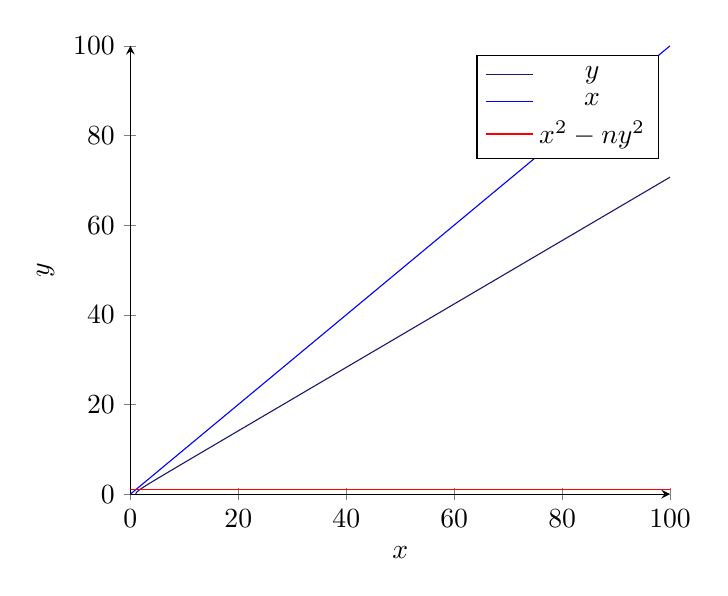
\begin{tikzpicture}
\begin{axis}[
    axis lines = left,
    xlabel = $x$,
    ylabel = {$y$},
]
\addplot [
    domain=0:100, 
    samples=1000, 
    color=MidnightBlue,
]
{((x^2 - 1)/2)^0.5};
\addlegendentry{$y$}
\addplot [
    domain=0:100, 
    samples=1000, 
    color=blue,
]
{x};
\addlegendentry{$x$}
\addplot [
    domain=0:100, 
    samples=1000, 
    color=red,
]
{1};
\addlegendentry{$x^2 - ny^2$}
\end{axis}
\end{tikzpicture}
\end{center}}
\end{mathbox}
%------------------------------------------------------------
\begin{chembox}{\text{\subsection{What are Subshells and Orbitals?}}}
{\textbf{Subshells:}\\
Each shell is composed of one or more subshells, which are themselves composed of atomic orbitals. For example, the first $(K)$ shell has one subshell, called $1s$; the second $(L)$ shell has two subshells, called $2s$ and $2p$; the third shell has $3s$, $3p$, and $3d$; the fourth shell has $4s$, $4p$, $4d$ and $4f$; the fifth shell has $5s$, $5p$, $5d$, and $5f$ and can theoretically hold more in the $5g$ subshell that is not occupied in the ground-state\footnote{The lowest energy state; i.e when the electron has very less energy to release or absorb.} electron configuration of any known element.
Each subshell is constrained to hold $4l$ + $2$ electrons at most, namely:
\begin{itemize}
    \item {Each $s$ subshell holds at most 2 electrons}
    \item{Each $p$ subshell holds at most 6 electrons}
    \item{Each $d$ subshell holds at most 10 electrons}
    \item{Each $f$ subshell holds at most 14 electrons}
    \item{Each $g$ subshell holds at most 18 electrons}
\end{itemize}
\textbf{Atomic Orbitals:}\\
In atomic theory and quantum mechanics, an atomic orbital is a mathematical function describing the location and wave-like behavior of an electron in an atom.This function can be used to calculate the probability of finding any electron of an atom in any specific region around the atom's nucleus. The term atomic orbital may also refer to the physical region or space where the electron can be calculated to be present, as predicted by the particular mathematical form of the orbital.
Orbitals have been given names, which are usually given in the form:\\
X orbital$^y$; where $X$ is the energy level corresponding to the principal quantum number $n$; type is a lower-case letter denoting the shape or subshell of the orbital, corresponding to the angular quantum number $l$; and $y$ is the number of electrons in that orbital.\\
For example, the orbital $1s^2$ (pronounced as the individual numbers and letters: "'one' 's' 'two'") has two electrons and is the lowest energy level $(n = 1)$ and has an angular quantum number of $l$ = 0, denoted by s.}
\end{chembox}
%------------------------------------------------------------
\begin{chembox}{\text{\subsection{Block Building Principle}}}
{The Aufbau principle, from the German "Aufbauprinzip" (building-up principle), also called the Aufbau rule, states that in the ground state of an atom or ion, electrons fill atomic orbitals of the lowest available energy levels before occupying higher levels. For example, the $1s$ subshell is filled before the $2s$ subshell is occupied. In this way, the electrons of an atom or ion form the most stable electron configuration possible. An example is the configuration $1s^2$ $2s^2$ $2p^6$ $3s^2$ $3p^3$ for the phosphorus atom, meaning that the $1s$ subshell has 2 electrons, and so on.

Electron behavior is elaborated by other principles of atomic physics, such as Hund's rule and the Pauli exclusion principle. Hund's rule asserts that if multiple orbitals of the same energy are available, electrons will occupy different orbitals singly before any are occupied doubly. If double occupation does occur, the Pauli exclusion principle requires that electrons that occupy the same orbital must have different spins. That is $\pm\frac{1}{2}$.
\begin{center}
    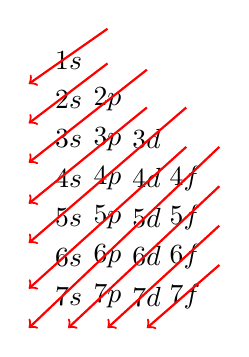
\begin{tikzpicture}
        \draw (-1,3) node[left] {$1s$};
        \draw (-1,2.5) node[left] {$2s$};
        \draw (-1,2) node[left] {$3s$};
        \draw (-1,1.5) node[left] {$4s$};
        \draw (-1,1) node[left] {$5s$};
        \draw (-1,0.5) node[left] {$6s$};
        \draw (-1,0) node[left] {$7s$};
        
        \draw (-0.5,2.5) node[left] {$2p$};
        \draw (-0.5,2) node[left] {$3p$};
        \draw (-0.5,1.5) node[left] {$4p$};
        \draw (-0.5,1) node[left] {$5p$};
        \draw (-0.5,0.51) node[left] {$6p$};
        \draw (-0.5,0) node[left] {$7p$};

        \draw (0,2) node[left] {$3d$};
        \draw (0,1.5) node[left] {$4d$};
        \draw (0,1) node[left] {$5d$};
        \draw (0,0.51) node[left] {$6d$};
        \draw (0,0) node[left] {$7d$};
        
        \draw (.5,1.5) node[left] {$4f$};
        \draw (.5,1) node[left] {$5f$};
        \draw (.5,0.51) node[left] {$6f$};
        \draw (.5,0) node[left] {$7f$};
        
        \draw[thick, ->, color=red] (-0.8, 3.4)->(-1.8,2.7);
        \draw[thick, ->, color=red] (-0.8, 2.96)->(-1.8,2.2);
        \draw[thick, ->, color=red] (-0.3, 2.88)->(-1.8,1.7);
        \draw[thick, ->, color=red] (-0.3, 2.4)->(-1.8,1.18);
        \draw[thick, ->, color=red] (0.2, 2.4)->(-1.8,0.68);
        \draw[thick, ->, color=red] (0.2, 1.9)->(-1.8,0.1);
        \draw[thick, ->, color=red] (0.62, 1.9)->(-1.8,-0.4);
        \draw[thick, ->, color=red] (0.62, 1.4)->(-1.3,-0.4);
        \draw[thick, ->, color=red] (0.62, 0.9)->(-0.8,-0.4);
        \draw[thick, ->, color=red] (0.62, 0.4)->(-0.3,-0.4);
    \end{tikzpicture}
\end{center}
A diagrammatic representation of the order to fill electron subshells.}
\end{chembox}
%------------------------------------------------------------
\begin{chembox}{\text{\subsection{Hund's Choco Orbital Rule}}}
{According to Hund’s rule:

Before the double occupation of any orbital, every orbital in the sub level is singly occupied.
For the maximization of total spin, all electrons in a single occupancy orbital have the same spin.
An electron will not pair with another electron in a half-filled orbital as it has the ability to fill all its orbitals with similar energy. Many unpaired electrons are present in atoms which are at the ground state. If two electrons come in contact they would show the same behaviour as two magnets do. The electrons first try to get as far away from each other as possible before they have to pair up.

The electrons enter an empty orbital before pairing up. The electrons repel each other as they are negatively charged. The electrons do not share orbitals to reduce repulsion.

When we consider the second rule, the spins of unpaired electrons in singly occupied orbitals are the same. The initial electrons spin in the sub-level decides what the spin of the other electrons would be. For instance, a carbon atom’s electron configuration would be $1s^2$ $2s^2$ $2p^2$. The same orbital will be occupied by the two 2s electrons although different orbitals will be occupied by the two $2p$ electrons in reference to Hund’s rule.}
\end{chembox}
%-------------------------------------------------------------
\begin{phybox}{\text{\subsection{Pauli's "Excluded" Principle}}}
{The Pauli's exclusion principle is the quantum mechanical principle which states that two or more identical fermions\footnote{Particles with half-integer spin} cannot occupy the same quantum state within a quantum system simultaneously. This principle was formulated by Austrian physicist Wolfgang Pauli in 1925 for electrons, and later extended to all fermions with his spin–statistics theorem of 1940.
In the case of electrons in atoms, it can be stated as follows: it is impossible for two electrons of a poly-electron atom to have the same values of the four quantum numbers: $n$, the principal quantum number, $l$, the azimuthal quantum number, $m$, the magnetic quantum number, and $s$, the spin quantum number. For example, if two electrons reside in the same orbital, then their $n$, $l$, and $m$ values are the same, therefore their $s$ must be different, and thus the electrons must have opposite half-integer spin projections of $\frac{1}{2}$ and $-\frac{1}{2}$.}
\end{phybox}
%-------------------------------------------------------------
\begin{phybox}{\text{\subsection{Half Life of Atoms}}}
{Half-life represented by $t_\frac{1}{2}$ is the time required for a quantity to reduce to half of its initial value. It’s used in nuclear physics to describe how quickly unstable atoms undergo radioactive decay or how long stable atoms survive. Half-life is mainly defined in terms of probability; i.e. ”Half-life is the time required for exactly half of the entities to decay on average”. In other words, the probability of a radioactive atom decaying within its half-life is 50%.\\
Exponential decay can be described by any of the following three equivalent formulas:
\begin{align*}
N(t)=N_{0}\left({\frac{1}{2}}\right)^{\frac{t}{t_{1/2}}}\\
N(t)=N_{0}e^{-{\frac {t}{\tau }}}\\
N(t)=N_{0}e^{-\lambda t}
\end{align*}
where;
\begin{itemize}
\item{$N_0$ is the initial quantity of the substance that will decay,}
\item{$N(t)$ is the quantity that still remains and has not yet decayed after a time $t$,}
\item{$t_\frac{1}{2}$ is the half-life of the decaying quantity, $\tau$ is a positive number called the mean lifetime of the decaying quantity,}
\item{$\lambda$ is a positive number called the decay constant of the decaying quantity.}
\end{itemize}
The three parameters $t_\frac{1}{2}$, $\tau$, and $\lambda$ are all directly related in the following way:
\begin{align*}
t_\frac{1}{2}={\frac {\ln(2)}{\lambda }}=\tau \ln(2)
\end{align*}}
\end{phybox} 
%------------------------------------------------------------
\newpage
%------------------------------------------------------------
